\section{Dark Matter models validations}
\label{sec:dm_checklist}

\subsection{\DMj models}

Tables~\ref{mostSensitiveBins_DMV_NNPDF30_Vector_Mphi-10_Mchi-1_gSM-1p0_gDM-1p0_25ns}-\ref{mostSensitiveBins_DMS_NNPDF30_Scalar_Mphi-500_Mchi-150_gSM-1p0_gDM-1p0_25ns} summarises the five most sensitive (\njet,\nb,\scalht,\mht) bins, background and signal yield and significance for selected \DMbb masses for two mass points each vor vector, axial-vector, pseudo-scalar and scalar samples

As expected, the sensitivity for these models mostly lies at low jet
multiplicities, low-medium \scalht, and at \mht values close to the upper bound
of the relevant \scalht bin Note that the \mht dimension is not utilised within 
the monojet category. Also note that, for convenience, all signal models have 
been normalised to a cross section of 10 pb in these tables.




\begin{tabular}{|l|l|l|l|l|}
\footnotesize
   \label{mostSensitiveBins_DMV_NNPDF30_Vector_Mphi-10_Mchi-1_gSM-1p0_gDM-1p0_25ns}
	\textbf{DMV NNPDF30 Vector Mphi-10 Mchi-1 gSM-1p0 gDM-1p0 25ns mht}	 & 	bgTtw	 & 	bgZinv	 & 	Signal &	 Significance \\ 
	\hline
	htBin 600-800 cat ge5j eq1b mht 350 & 	2.43	 & 	1.16	 & 	0.00 	&0.000000 \\ 
	htBin 800-Inf cat ge5j eq0b mht 575 & 	0.55	 & 	1.71	 & 	0.00 	&0.000000 \\ 
	htBin 600-Inf cat eq4a eq1b mht 575 & 	0.02	 & 	0.08	 & 	0.00 	&0.000000 \\ 
	htBin 350-400 cat eq4j eq1b mht 0 & 	5.05	 & 	0.75	 & 	0.00 	&0.000000 \\ 
	htBin 350-400 cat ge5j eq1b mht 0 & 	2.24	 & 	0.28	 & 	0.00 	&0.000000 \\ 
\end{tabular}
\\
 \begin{tabular}{|l|l|l|l|l|}
\small
   \label{mostSensitiveBins_DMV_NNPDF30_Vector_Mphi-500_Mchi-150_gSM-1p0_gDM-1p0_25ns}
	\textbf{DMV NNPDF30 Vector Mphi-500 Mchi-150 gSM-1p0 gDM-1p0}	 & 	bgTtw	 & 	bgZinv	 & 	Signal &	 Significance \\ 
	\hline
	htBin 600-800 cat eq3j eq1b mht 525 & 	0.35	 & 	1.08	 & 	0.60 	&0.376317 \\ 
	htBin 800-Inf cat eq3j eq0b mht 575 & 	0.99	 & 	2.64	 & 	0.52 	&0.166584 \\ 
	htBin 800-Inf cat eq3j eq0b mht 425 & 	1.40	 & 	4.20	 & 	0.57 	&0.137786 \\ 
	htBin 400-500 cat eq2j eq1b mht 375 & 	2.48	 & 	4.18	 & 	0.40 	&0.102571 \\ 
	htBin 500-600 cat eq2j eq1b mht 575 & 	0.33	 & 	0.56	 & 	0.38 	&0.084309 \\ 
\end{tabular}
\\

 \begin{tabular}{|l|l|l|l|l|}
\small
   \label{mostSensitiveBins_DMV_NNPDF30_Axial_Mphi-10_Mchi-1_gSM-1p0_gDM-1p0_25ns}
   \textbf{DMV NNPDF30 Axial Mphi-10 Mchi-1 gSM-1p0 gDM-1p0}	 a& 	bgTtw	 & 	bgZinv	 & 	Signal &	 Significance \\ 
	\hline
	htBin 200-250 cat eq3a ge3b mht 0 & 	0.50	 & 	0.08	 & 	0.00 	&0.000000 \\ 
	htBin 600-800 cat ge5j eq1b mht 350 & 	2.43	 & 	1.16	 & 	0.00 	&0.000000 \\ 
	htBin 800-Inf cat ge5j eq0b mht 575 & 	0.55	 & 	1.71	 & 	0.00 	&0.000000 \\ 
	htBin 600-Inf cat eq4a eq1b mht 575 & 	0.02	 & 	0.08	 & 	0.00 	&0.000000 \\ 
	htBin 350-400 cat eq4j eq1b mht 0 & 	5.05	 & 	0.75	 & 	0.00 	&0.000000 \\ 
\end{tabular}
\\
 \begin{tabular}{|l|l|l|l|l|}
  \small
\label{mostSensitiveBins_DMV_NNPDF30_Axial_Mphi-500_Mchi-150_gSM-1p0_gDM-1p0_25ns}
	\textbf{DMV NNPDF30 Axial Mphi-500 Mchi-150 gSM-1p0 gDM-1p0}	 & 	bgTtw	 & 	bgZinv	 & 	Signal &	 Significance \\ 
	\hline
	htBin 600-800 cat eq4j eq0b mht 550 & 	1.12	 & 	3.44	 & 	0.72 	&0.174754 \\ 
	htBin 400-500 cat eq2a eq0b mht 475 & 	4.52	 & 	9.61	 & 	1.61 	&0.150429 \\ 
	htBin 500-600 cat eq3a eq0b mht 525 & 	1.02	 & 	2.66	 & 	0.40 	&0.140377 \\ 
	htBin 800-Inf cat ge5j eq1b mht 475 & 	0.46	 & 	0.40	 & 	0.33 	&0.105422 \\ 
	htBin 500-600 cat eq2a eq0b mht 0 & 	4.09	 & 	9.48	 & 	0.73 	&0.077469 \\ 
\end{tabular}
\\

\begin{tabular}{|l|l|l|l|l|}
\small
  \label{mostSensitiveBins_DMS_NNPDF30_Pseudoscalar_Mphi-10_Mchi-1_gSM-1p0_gDM-1p0_25ns}
	\textbf{DMS NNPDF30 Pseudoscalar Mphi-10 Mchi-1 gSM-1p0 gDM-1p0}	 & 	bgTtw	 & 	bgZinv	 & 	Signal &	 Significance \\ 
	\hline
	htBin 250-300 cat eq2a eq0b mht 275 & 	127.65	 & 	198.28	 & 	0.09 	&0.000725 \\ 
	htBin 200-250 cat eq3a eq0b mht 175 & 	382.80	 & 	352.12	 & 	0.10 	&0.000369 \\ 
	htBin 250-300 cat eq1j eq0b mht 0 & 	1334.66	 & 	2272.06	 & 	0.84 	&0.000257 \\ 
	htBin 200-250 cat eq2a eq0b mht 175 & 	1587.13	 & 	1778.80	 & 	0.35 	&0.000070 \\ 
	htBin 250-300 cat eq2j eq0b mht 225 & 	211.65	 & 	271.34	 & 	0.32 	&0.000061 \\ 
\end{tabular}
\\
\begin{tabular}{|l|l|l|l|l|}
\small
  \label{mostSensitiveBins_DMS_NNPDF30_Pseudoscalar_Mphi-500_Mchi-150_gSM-1p0_gDM-1p0_25ns}
	\textbf{DMS NNPDF30 Pseudoscalar Mphi-500 Mchi-150 gSM-1p0 gDM-1p0}	 & 	bgTtw	 & 	bgZinv	 & 	Signal &	 Significance \\ 
	\hline
	htBin 250-300 cat eq2j eq1b mht 0 & 	1.04	 & 	0.60	 & 	0.37 	&0.217363 \\ 
	htBin 800-Inf cat ge5j eq1b mht 525 & 	0.36	 & 	0.35	 & 	0.35 	&0.216671 \\ 
	htBin 600-800 cat ge5j eq0b mht 475 & 	1.14	 & 	2.47	 & 	0.70 	&0.176768 \\ 
	htBin 500-600 cat eq3a eq0b mht 525 & 	1.02	 & 	2.66	 & 	0.36 	&0.140377 \\ 
	htBin 600-800 cat eq3j eq1b mht 475 & 	0.93	 & 	0.91	 & 	0.19 	&0.097086 \\ 
\end{tabular}
\\

 \begin{tabular}{|l|l|l|l|l|}
\small
   \label{mostSensitiveBins_DMS_NNPDF30_Scalar_Mphi-10_Mchi-1_gSM-1p0_gDM-1p0_25ns}
	\textbf{DMS NNPDF30 Scalar Mphi-10 Mchi-1 gSM-1p0 gDM-1p0}	 & 	bgTtw	 & 	bgZinv	 & 	Signal &	 Significance \\ 
	\hline
	htBin 400-500 cat eq1j eq1b mht 0 & 	5.46	 & 	11.40	 & 	0.18 	&0.020358 \\ 
	htBin 200-250 cat eq2a eq0b mht 175 & 	1587.13	 & 	1778.80	 & 	0.39 	&0.000070 \\ 
	htBin 250-300 cat eq2j eq0b mht 225 & 	211.65	 & 	271.34	 & 	0.05 	&0.000061 \\ 
	htBin 200-250 cat eq1j eq0b mht 0 & 	4336.68	 & 	6239.23	 & 	0.64 	&0.000028 \\ 
	htBin 200-250 cat eq3a ge3b mht 0 & 	0.50	 & 	0.08	 & 	0.00 	&0.000000 \\ 
\end{tabular}

\\
 \begin{tabular}{|l|l|l|l|l|}
\small
   \label{mostSensitiveBins_DMS_NNPDF30_Scalar_Mphi-500_Mchi-150_gSM-1p0_gDM-1p0_25ns}
	\textbf{DMS NNPDF30 Scalar Mphi-500 Mchi-150 gSM-1p0 gDM-1p0 25ns mht}	 & 	bgTtw	 & 	bgZinv	 & 	Signal &	 Significance \\ 
	\hline
	htBin 600-800 cat eq2j eq0b mht 725 & 	0.38	 & 	1.30	 & 	0.36 	&0.203516 \\ 
	htBin 600-800 cat eq4j eq0b mht 550 & 	1.12	 & 	3.44	 & 	0.64 	&0.174754 \\ 
	htBin 800-Inf cat eq4j eq0b mht 675 & 	0.52	 & 	1.24	 & 	0.28 	&0.152232 \\ 
	htBin 600-800 cat eq4j eq0b mht 650 & 	0.43	 & 	1.35	 & 	0.28 	&0.140296 \\ 
	htBin 350-400 cat eq2j eq1b mht 325 & 	3.81	 & 	4.75	 & 	0.46 	&0.109951 \\ 
\end{tabular}
\\



\clearpage
\subsection{\DMbb and \DMtt models}



Tables~\ref{mostSensitiveBins_BBbarDMJets_pseudoscalar_Mchi-1_Mphi-10_25ns}-\ref{mostSensitiveBins_BBbarDMJets_scalar_Mchi-150_Mphi-500_25ns}.
show the five most sensitive bins, background and signal yield and significance for selected \DMbb masses.

 \begin{tabular}{|l|l|l|l|l|}
\small
   \label{mostSensitiveBins_BBbarDMJets_pseudoscalar_Mchi-1_Mphi-10_25ns}
	\textbf{BBbarDMJets pseudoscalar Mchi-1 Mphi-10}	 & 	bgTtw	 & 	bgZinv	 & 	Signal &	 Significance \\ 
	\hline
	htBin 200-250 cat eq1j eq0b mht 0 & 	4336.68	 & 	6239.23	 & 	0.18 	&0.000028 \\ 
	htBin 200-250 cat eq3a ge3b mht 0 & 	0.50	 & 	0.08	 & 	0.00 	&0.000000 \\ 
	htBin 600-800 cat ge5j eq1b mht 350 & 	2.43	 & 	1.16	 & 	0.00 	&0.000000 \\ 
	htBin 800-Inf cat ge5j eq0b mht 575 & 	0.55	 & 	1.71	 & 	0.00 	&0.000000 \\ 
	htBin 600-Inf cat eq4a eq1b mht 575 & 	0.02	 & 	0.08	 & 	0.00 	&0.000000 \\ 
\end{tabular}

\\
 \begin{tabular}{|l|l|l|l|l|}
\small
   \label{mostSensitiveBins_BBbarDMJets_pseudoscalar_Mchi-150_Mphi-500_25ns}
	\textbf{BBbarDMJets pseudoscalar Mchi-150 Mphi-500}	 & 	bgTtw	 & 	bgZinv	 & 	Signal &	 Significance \\ 
	\hline
	htBin 350-400 cat eq4a eq1b mht 300 & 	2.34	 & 	1.27	 & 	1.50 	&0.603291 \\ 
	htBin 200-250 cat eq2a eq2b mht 175 & 	8.86	 & 	7.42	 & 	4.29 	&0.571712 \\ 
	htBin 400-500 cat ge5a eq2b mht 250 & 	1.91	 & 	0.13	 & 	1.20 	&0.568945 \\ 
	htBin 250-300 cat eq2a eq2b mht 0 & 	2.01	 & 	1.76	 & 	1.24 	&0.532145 \\ 
	htBin 350-400 cat eq3a eq1b mht 275 & 	3.33	 & 	3.01	 & 	1.66 	&0.513233 \\ 
\end{tabular}
\\
 \begin{tabular}{|l|l|l|l|l|}
\small
   \label{mostSensitiveBins_BBbarDMJets_scalar_Mchi-1_Mphi-10_25ns}
	\textbf{BBbarDMJets scalar Mchi-1 Mphi-10}	 & 	bgTtw	 & 	bgZinv	 & 	Signal &	 Significance \\ 
	\hline
	htBin 600-800 cat ge5j eq1b mht 350 & 	2.43	 & 	1.16	 & 	0.00 	&0.000000 \\ 
	htBin 800-Inf cat ge5j eq0b mht 575 & 	0.55	 & 	1.71	 & 	0.00 	&0.000000 \\ 
	htBin 600-Inf cat eq4a eq1b mht 575 & 	0.02	 & 	0.08	 & 	0.00 	&0.000000 \\ 
	htBin 350-400 cat eq4j eq1b mht 0 & 	5.05	 & 	0.75	 & 	0.00 	&0.000000 \\ 
	htBin 800-Inf cat eq3j eq1b mht 675 & 	0.04	 & 	0.21	 & 	0.00 	&0.000000 \\ 
\end{tabular}
\\
 \begin{tabular}{|l|l|l|l|l|}
\small
   \label{mostSensitiveBins_BBbarDMJets_scalar_Mchi-150_Mphi-500_25ns}
	\textbf{BBbarDMJets scalar Mchi-150 Mphi-500}	 & 	bgTtw	 & 	bgZinv	 & 	Signal &	 Significance \\ 
	\hline
	htBin 200-250 cat eq2j eq2b mht 0 & 	0.97	 & 	0.93	 & 	2.28 	&1.273182 \\ 
	htBin 250-300 cat eq3a eq2b mht 250 & 	1.45	 & 	0.92	 & 	1.72 	&0.897552 \\ 
	htBin 400-500 cat eq3j eq1b mht 425 & 	1.60	 & 	1.72	 & 	1.81 	&0.789506 \\ 
	htBin 400-500 cat eq3j eq1b mht 275 & 	7.15	 & 	6.38	 & 	3.67 	&0.619530 \\ 
	htBin 500-600 cat ge5j ge3b mht 0 & 	1.13	 & 	0.04	 & 	1.20 	&0.579402 \\ 
\end{tabular}
\\

Most sensitive bins are large ($b$)-jet multiplicities, medium to high \scalht and \mht values. Note that, for convenience, all signal models have been normalised to a cross section of 10 pb in these tables.

\clearpage

Background and signal yields for the most sensitive bins for \DMtt samples are given in Tables~\ref{mostSensitiveBins_TTbarDMJets_pseudoscalar_Mchi-1_Mphi-10_25ns}-\ref{mostSensitiveBins_TTbarDMJets_scalar_Mchi-150_Mphi-500_25ns}.

As expected, the sensitivity for these models mostly lies at large jet and $b$-jet multiplicities, high \scalht as well as large \mht values. Also these tablesa are all normalised to $\sigma=10$\ipb


\begin{tabular}{|l|l|l|l|l|}
  \small
   \label{mostSensitiveBins_TTbarDMJets_pseudoscalar_Mchi-1_Mphi-10_25ns}
	\textbf{TTbarDMJets pseudoscalar Mchi-1 Mphi-10}	 & 	bgTtw	 & 	bgZinv	 & 	Signal &	 Significance \\ 
	\hline
	htBin 400-500 cat ge5j eq1b mht 300 & 	2.30	 & 	0.59	 & 	8.27 	&4.084547 \\ 
	htBin 600-800 cat ge5j eq2b mht 425 & 	0.19	 & 	0.04	 & 	5.54 	&3.958966 \\ 
	htBin 600-800 cat ge5j eq1b mht 450 & 	0.59	 & 	0.40	 & 	5.24 	&3.556865 \\ 
	htBin 400-500 cat ge5j eq2b mht 325 & 	0.43	 & 	0.08	 & 	5.05 	&3.519975 \\ 
	htBin 350-400 cat ge5a eq1b mht 300 & 	0.29	 & 	0.23	 & 	4.50 	&3.476202 \\ 
\end{tabular}
\\
 \begin{tabular}{|l|l|l|l|l|}
  \small
   \label{mostSensitiveBins_TTbarDMJets_pseudoscalar_Mchi-150_Mphi-500_25ns}
	\textbf{TTbarDMJets pseudoscalar Mchi-150 Mphi-500}	 & 	bgTtw	 & 	bgZinv	 & 	Signal &	 Significance \\ 
	\hline
	htBin 600-800 cat ge5j eq1b mht 450 & 	0.59	 & 	0.40	 & 	35.12 	&24.867541 \\ 
	htBin 800-Inf cat ge5j eq1b mht 775 & 	0.09	 & 	0.39	 & 	23.55 	&18.646455 \\ 
	htBin 600-800 cat ge5j eq2b mht 325 & 	0.60	 & 	0.12	 & 	24.68 	&18.190695 \\ 
	htBin 600-800 cat ge5j eq1b mht 500 & 	0.27	 & 	0.34	 & 	23.81 	&18.032253 \\ 
	htBin 600-800 cat ge5j eq1b mht 400 & 	1.67	 & 	0.69	 & 	30.89 	&17.157983 \\ 
\end{tabular}
\\
\begin{tabular}{|l|l|l|l|l|}
\small
   \label{mostSensitiveBins_TTbarDMJets_scalar_Mchi-1_Mphi-10_25ns}
	\textbf{TTbarDMJets scalar Mchi-1 Mphi-10}	 & 	bgTtw	 & 	bgZinv	 & 	Signal &	 Significance \\ 
	\hline
	htBin 600-800 cat ge5j eq2b mht 275 & 	1.49	 & 	0.25	 & 	1.34 	&0.789106 \\ 
	htBin 350-400 cat eq3j eq2b mht 300 & 	0.85	 & 	0.13	 & 	1.33 	&0.717537 \\ 
	htBin 800-Inf cat ge5j eq1b mht 425 & 	0.63	 & 	0.41	 & 	1.32 	&0.676182 \\ 
	htBin 400-500 cat ge5a eq2b mht 200 & 	5.24	 & 	0.20	 & 	2.12 	&0.543026 \\ 
	htBin 400-500 cat eq4j eq1b mht 300 & 	7.80	 & 	2.75	 & 	2.54 	&0.532218 \\ 
\end{tabular}
\\
 \begin{tabular}{|l|l|l|l|l|}
\small
\label{mostSensitiveBins_TTbarDMJets_scalar_Mchi-150_Mphi-500_25ns}
	\textbf{TTbarDMJets scalar Mchi-150 Mphi-500}	 & 	bgTtw	 & 	bgZinv	 & 	Signal &	 Significance \\ 
	\hline
	htBin 800-Inf cat ge5j eq2b mht 725 & 	0.23	 & 	0.08	 & 	25.79 	&20.939012 \\ 
	htBin 600-800 cat ge5j eq2b mht 375 & 	0.47	 & 	0.13	 & 	26.05 	&19.598534 \\ 
	htBin 800-Inf cat ge5j eq1b mht 775 & 	0.09	 & 	0.39	 & 	24.14 	&18.646455 \\ 
	htBin 600-800 cat ge5j eq2b mht 525 & 	0.49	 & 	0.09	 & 	23.75 	&17.972944 \\ 
	htBin 600-800 cat ge5j eq2b mht 325 & 	0.60	 & 	0.12	 & 	20.36 	&15.194035 \\ 
\end{tabular}
\\



\clearpage

\subsection{Best limits per jet category}

The best limits for each jet category are given in Tables~\ref{MSBAxialVector0p25},~\ref{MSBPseudoScalar} for various meditator and DM masses. It has to be pointed out that 
the all cross sections are normalied to 10pb.

\begin{table*}
\begin{center}
\caption{Axial vector gSM=0.25, gDM=1, r-values for each Njet category}
\footnotesize
\begin{tabular}{cc|lllllll}\hline 
\label{MSBAxialVector0p25}
\mphi & \mchi & monojet & 2j asym. & 2j sym.  & 3j asym. &3j sym. & 4j asym.  & 4j sym. \\ \hline
10    & 50  & 37.95  & 44.38  & 12.41 & 69.81  & 12.81 & 14.38 & 14.56 \\
10    & 100 & 17.95  & 10.34  & 9.78  & 20.19  & 5.92  & 19.63 & 12.41 \\
10    & 500 & 1.77   & 3.67   & 1.41  & 2.63   & 1.36  & 2.98  & 1.73  \\
100   & 1   & 141.25 & 344.75 & 56.25 & 61.63  & 55.25 &       & 29.13 \\
100   & 10  & 89.25  & 53.91  & 54.63 & 126.25 & 19.31 &       & 37.13 \\
100   & 100 & 14.38  & 9.41   & 4.89  & 5.17   & 5.70  & 3.39  & 7.59  \\
200   & 1   & 36.95  & 13.06  & 11.66 & 37.94  & 17.06 & 19.19 & 7.41  \\
200   & 10  & 41.13  & 27.63  & 14.81 & 25.95  & 8.84  & 52.50 & 47.63 \\
200   & 150 & 8.34   & 4.02   & 5.30  & 3.63   & 4.23  & 8.09  & 5.02  \\
300   & 1   & 16.31  & 22.81  & 6.20  & 17.44  & 8.41  & 22.56 & 10.03 \\
300   & 150 & 12.94  & 9.53   & 5.39  & 10.91  & 5.05  & 37.38 & 4.48  \\
500   & 1   & 6.34   & 8.50   & 5.36  & 5.30   & 6.02  & 4.98  & 5.70  \\
500   & 50  & 5.27   & 7.91   & 5.20  & 9.78   & 4.05  & 5.02  & 3.52  \\
500   & 100 & 6.22   & 12.28  & 3.14  & 3.61   & 4.83  & 7.41  & 3.98  \\
500   & 500 & 1.63   & 2.93   & 1.39  & 2.07   & 1.02  & 3.73  & 2.45  \\
1000  & 50  & 2.79   & 2.71   & 1.88  & 3.05   & 1.54  & 3.13  & 3.30  \\
1000  & 150 & 2.87   & 3.05   & 1.68  & 4.20   & 2.41  & 5.33  & 2.79  \\
1000  & 500 & 2.09   & 1.99   & 1.54  & 1.48   & 1.73  & 2.55  & 2.48  \\
2000  & 50  & 1.23   & 3.04   & 1.39  & 2.49   & 1.36  & 3.13  & 1.62  \\
10000 & 1   & 3.33   & 4.67   & 1.99  & 4.14   & 2.02  & 3.98  & 4.11  \\
10000 & 100 & 2.41   & 2.55   & 1.71  & 2.45   & 1.77  & 3.45  & 2.15  \\
10000 & 150 & 2.13   & 3.92   & 1.60  & 3.64   & 2.35  & 2.04  & 1.79  \\ \hline
\end{tabular}
\end{center}
\end{table*}


\\

\begin{table*}
\begin{center}
\caption{Pseudoscalar gSM=1, gDM=1, r-values for each Njet category}
\footnotesize
\begin{tabular}{cc|lllllll}\hline 
\label{MSBPseudoScalar}
\mphi & \mchi & monojet & 2j asym. & 2j sym.  & 3j asym. &3j sym. & 4j asym.  & 4j sym. \\ \hline
10000&1000&  2.1016& 2.125 &  0.7168& 2.2578&  0.752&1.7109&  0.7852\\
10000&100&  15.1875& 9.5&  6.0469& 5.2031&  3.0234&7.0&  4.0469\\
10000&10&  8.9531& 4.9219&  4.4844& 8.7812&  5.0156&6.8438&  6.3438\\
10000&150&  8.3438& 8.0312&  3.0391& 5.5469&  3.6406&7.4688&  3.7344\\
10000&1&  12.6875& 8.2188&  5.6094& 10.4062&  2.9609&10.8438&  2.3516\\
10000&500&  4.0469& 3.8906&  2.0234& 1.7891&  1.4883&1.9609&  1.1836\\
10000&50&  13.4062& 12.0938&  3.8906& 6.6562&  4.4531&7.6562&  3.3594\\
1000&1000&  2.1641& 3.0703&  0.9414& 1.7734&  0.9336&1.8359&  0.7852\\
1000&100&  7.5938& 5.2656&  2.5234& 5.9531&  2.1953&5.8594&  2.5234\\
1000&10&  7.0938& 4.2656&  3.1719& 4.2656&  2.9062&3.7031&  2.6953\\
1000&150&  5.7969& 7.1562&  2.3125& 2.8203&  2.4297&5.2344&  2.0234\\
1000&1&  7.4531& 4.6094&  3.2969& 4.25&  2.1016&4.0156&  1.9141\\
1000&500&  4.8281& 5.8594&  2.5938& 4.2969&  1.8047&5.5469&  1.8828\\
1000&50&  5.7656& 6.1406&  2.5234& 5.1719&  2.4766&3.2031&  2.4141\\
100&100&  24.0625& 15.0625&  5.2031& 9.8438&  8.2188&9.0312&  8.5312\\
100&10&  103.25& 59.25&  19.5625& 40.375&  23.0625&21.9688&  12.4062\\
100&50&  19.9766& 12.1875&  12.6875& 18.1875&  14.4375&62.25&  8.5938\\
10&10&  68.8125& 40.625&  35.8125& 17.1875&  46.375&28.375&  24.625\\
10&1&& 116.25&  131.25& 334.25&  30.375&&\\
2000&1000&  2.1797& 2.3672&  0.8242& 2.4922&  0.7852&2.2734&  1.1992\\
2000&10&  4.2031& 4.3906&  2.5547& 3.6719&  2.2109&2.9219&  2.0234\\
2000&150&  4.3906& 5.9766&  1.6016& 3.0703&  1.5352&3.3906&  1.3555\\
2000&1&  4.4531& 5.2344&  1.9297& 3.0234&  1.8672&3.7344&  1.8359\\
2000&500&  2.7266& 2.7266&  1.3711& 2.2266&  0.9102&2.4766&  1.0039\\
2000&50&  5.0469& 3.5469&  1.8516& 3.4219&  1.5586&2.9297&  2.2578\\
200&100&  34.125& 37.625&  12.5& 13.4375&  6.8125&12.8125&  10.5938\\
200&10&  50.625& 13.5625&  8.7188& 12.6875&  10.9062&11.4062&  20.8125\\
200&150&  13.3125& 18.5625&  7.2188& 12.8125&  4.0156&8.7812&  6.3438\\
200&1&  35.375& 41.75&  8.1562& 16.6875&  11.0312&12.3438&  9.6562\\
200&50&  34.375& 19.9688&  19.4375& 11.9531&  10.1562&16.0625&  7.2812\\
20&10&  322.625& 147.5&  28.625& 38.625&  58.625&75.25&  56.75\\
20&1&& 156.625&  32.625& 80.25&  29.125&149.25&  59.25\\
300&100&  27.125& 17.6875&  13.6875& 15.8125&  11.0312&10.1562&  20.8125\\
300&10&  28.375& 21.4375&  13.8125& 14.5625&  9.9531&18.4375&  11.6562\\
300&150&  20.1875& 24.4375&  8.4688& 14.0625&  7.4688&6.7812&  11.9062\\
300&50&  32.375& 28.125&  10.0312& 12.5625&  8.0938&8.2812&  8.2188\\
5000&1000&  1.5703& 2.3516&  0.8789& 1.6016&  0.7812&1.4961&  0.6152\\
5000&100&  10.7812& 6.4531&  4.3281& 4.2656&  2.8516&3.7969&  4.7969\\
5000&10&  11.8438& 6.1094&  5.8594& 4.5781&  4.0469&12.2188&  4.5469\\
5000&150&  8.5312& 6.9531&  4.2656& 3.8281&  2.2266&9.5938&  3.1172\\
5000&1&  12.8125& 9.2188&  3.2656& 8.0312&  3.6406&8.0938&  3.9531\\
5000&500&  3.1719& 3.2969&  1.543& 2.6016&  1.3945&2.8672&  1.1523\\
5000&50&  10.0312& 6.4062&  4.6719& 6.6562&  3.8906&6.4688&  3.0703\\
500&100&  15.4062& 7.3438&  3.8594& 17.75&  3.3906&7.4688&  4.2031\\
500&10&  14.9883& 9.4766&  7.0312& 17.6875&  3.2031&7.6562&  6.4688\\
500&150&  14.6875& 17.1875&  7.1562& 7.6562&  4.9062&10.8438&  7.2188\\
500&1&  16.8125& 10.0938&  5.6406& 10.1562&  4.0469&9.8438&  3.3594\\
500&500&  6.3438& 3.6094&  1.9141& 2.7109&  1.5508&2.3984&  2.0859\\
500&50&  20.5625& 10.3438&  5.2344& 7.0312&  5.0781&6.7188&  7.4688\\
50&10&  200.75& 50.0213&  41.25& 79.9531&  52.9531&142.25&  36.625\\
50&1&  59.875& 128.25&  64.25& 31.125&  73.25&40.9062&\\
50&50&  31.625& 19.9062&  11.3438& 18.9062&  8.0312& 10.8125&  16.5625\\ \hline
\end{tabular}
\end{center}
\end{table*}


%\begin{minipage}[b]{1\linewidth}
%\centering
%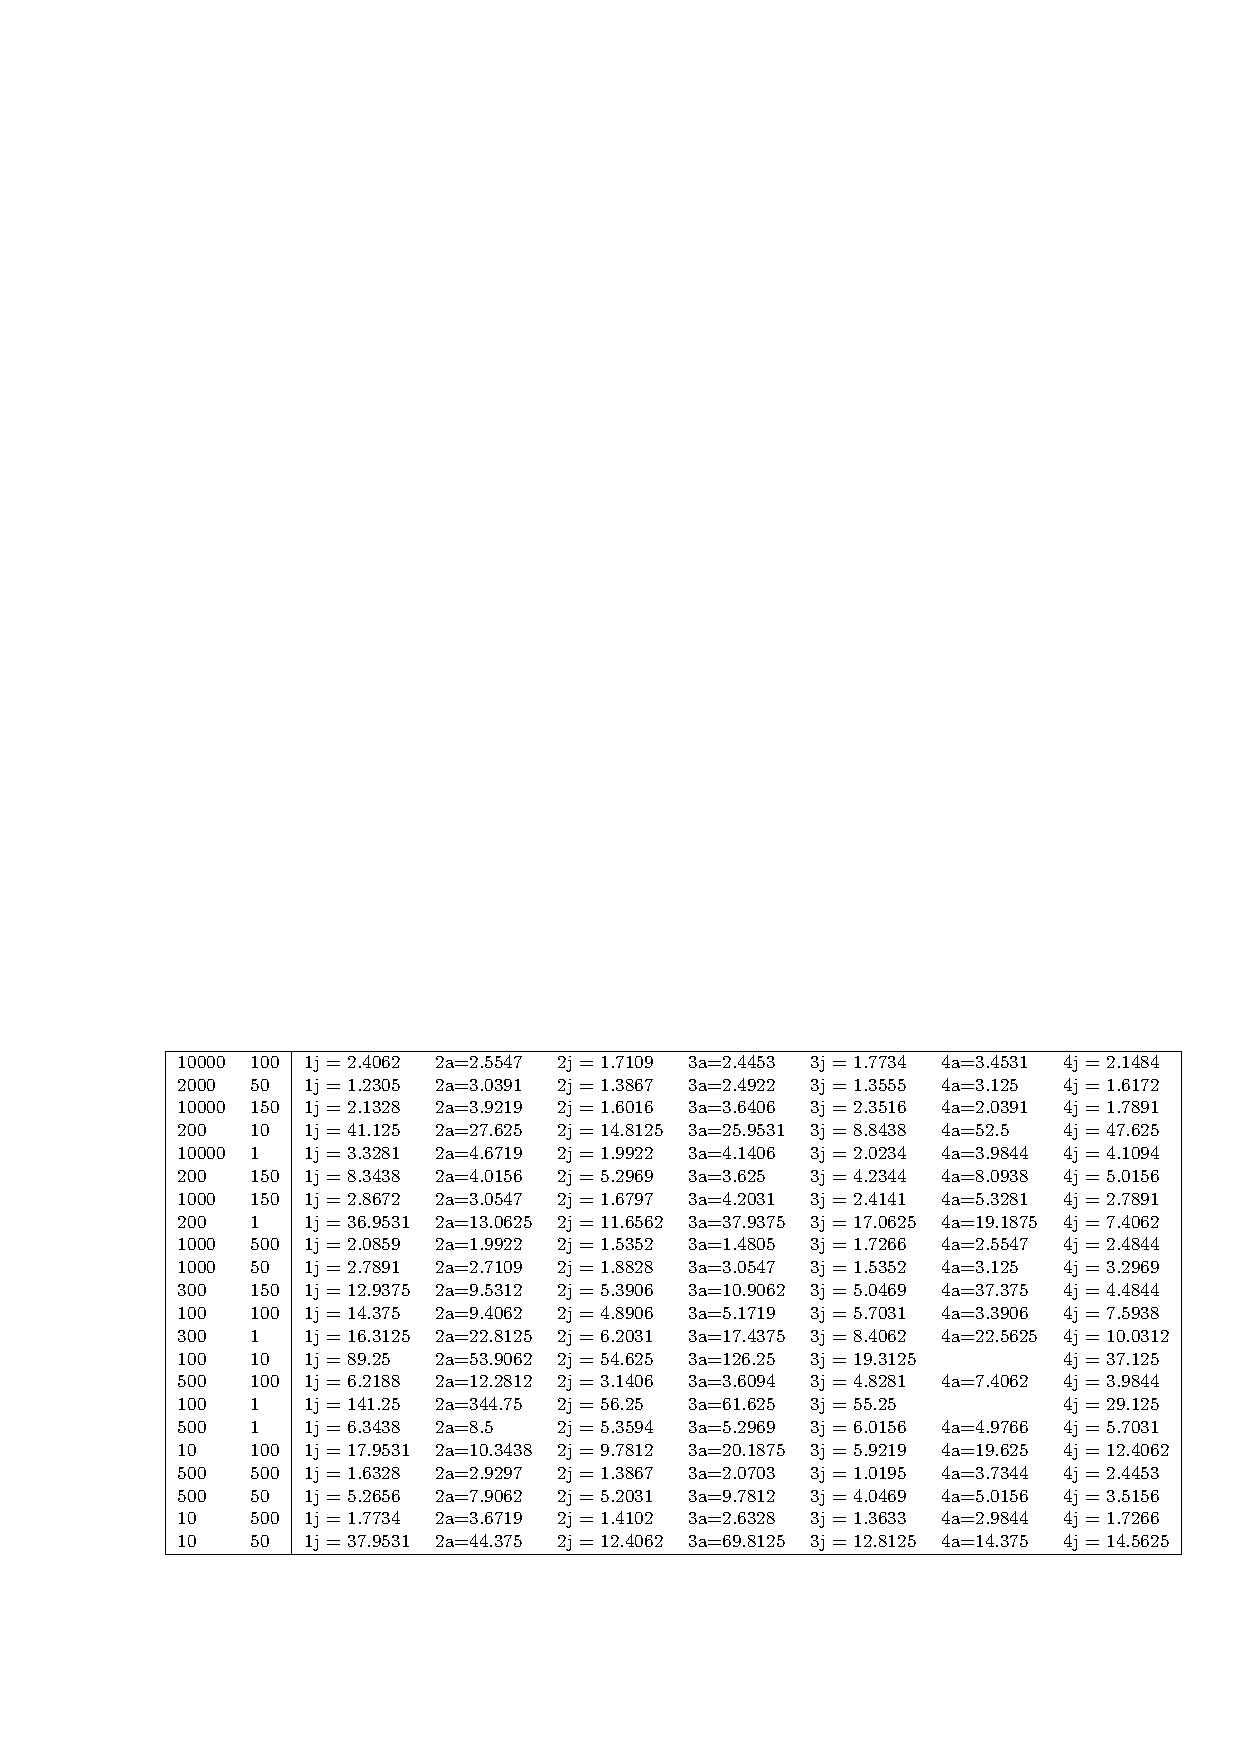
\includegraphics[scale=0.95]{tables/DM/AxialvectorMSNjet0p25.pdf}
%\label{tab:best_cat_a}

%\end{minipage}


%\begin{minipage}[b]{1\linewidth}
%\centering
%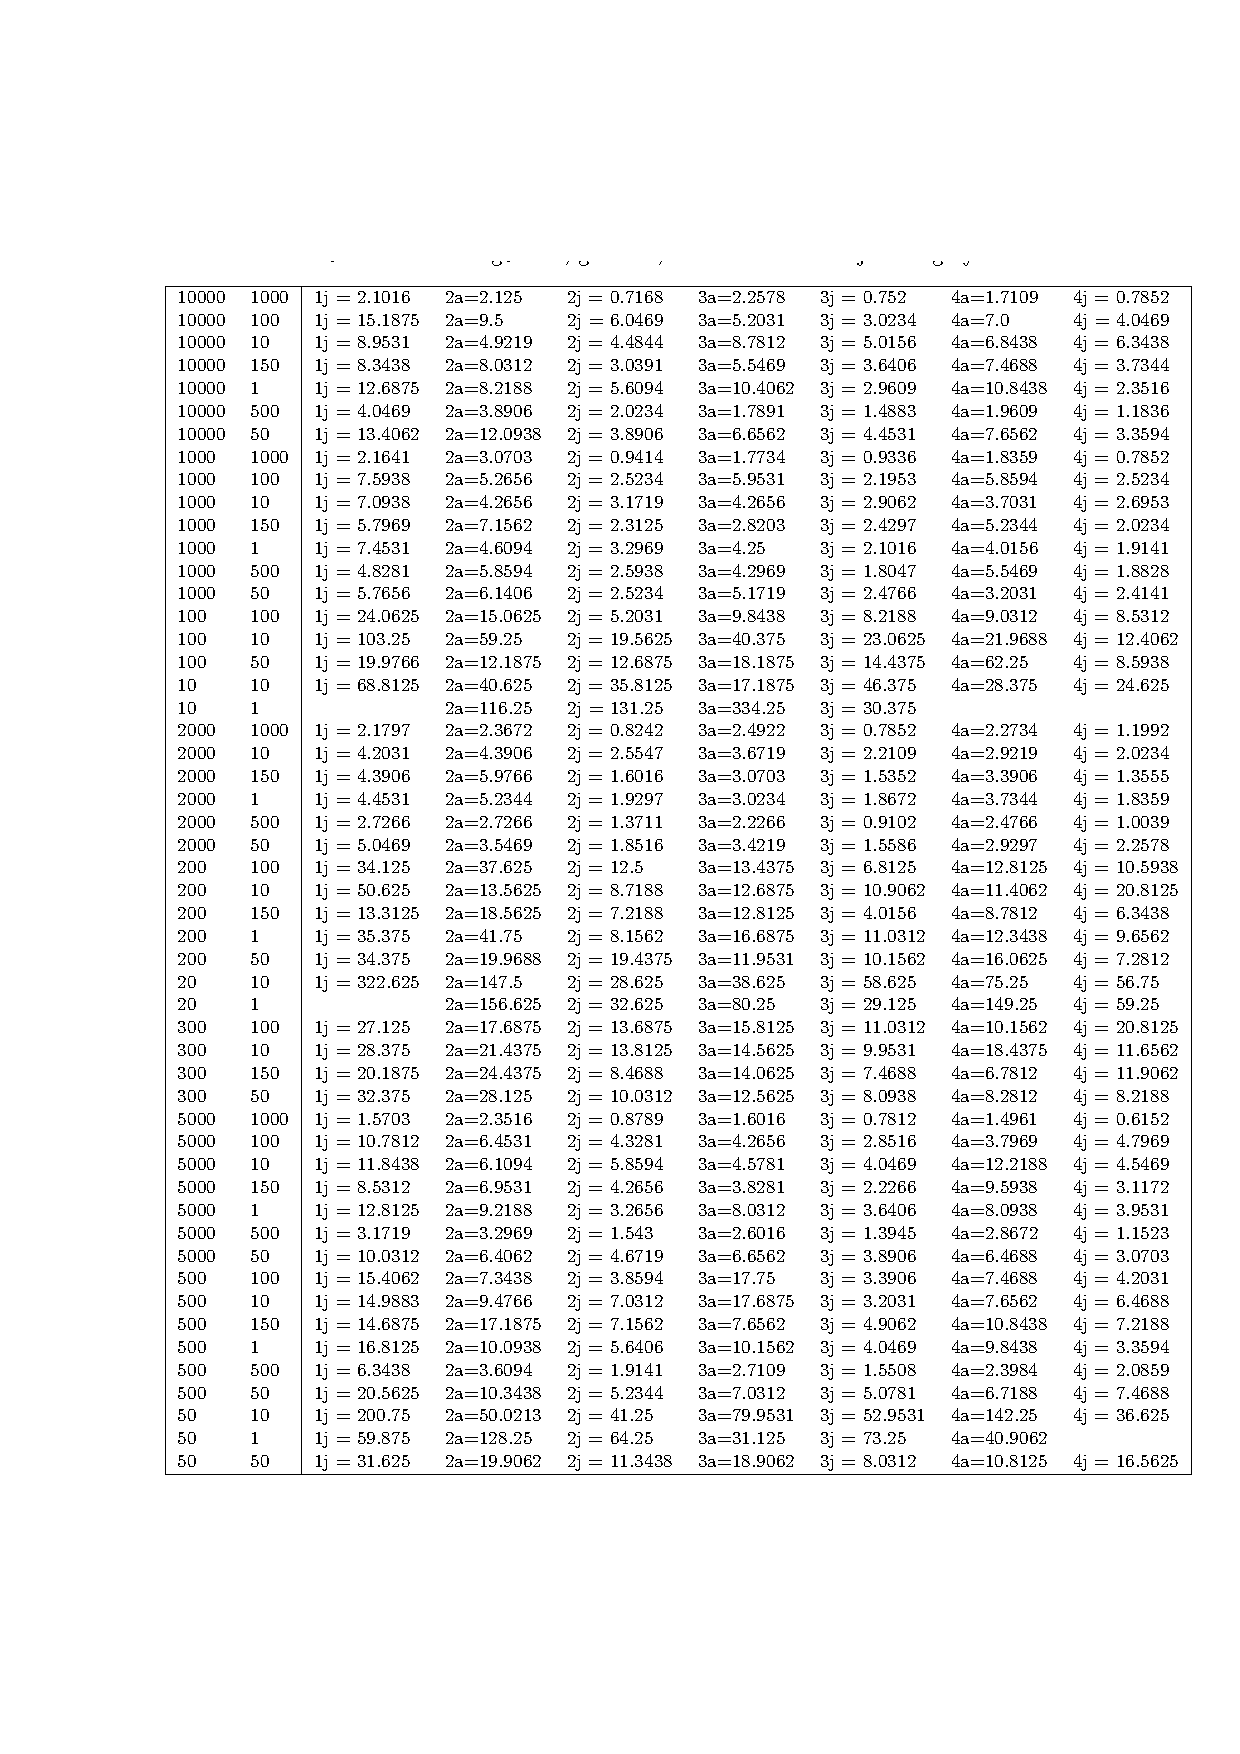
\includegraphics[scale=0.95]{tables/DM/PseudoscalarMSNjet.pdf}
%\label{tab:best_cat_p}
%\captionof{table}{Best sensitivity per jet selection for the axial pseudo-scalar samples. The production crosssections are normalised to 10pb}
%\end{minipage}
